\documentclass[12pt]{article}
\usepackage{mathrsfs}
\usepackage{graphicx,subfigure,setspace,lscape,longtable}
\usepackage{epsfig,graphicx}
\usepackage{mathrsfs,amsmath,amsthm,amssymb,color,bm}
\usepackage{booktabs}
\usepackage{hyperref}
\usepackage{amsfonts}
\usepackage{array,multirow}
\usepackage{caption}
\usepackage{float}
%\usepackage[round,colon,authoryear]{natbib}
\usepackage{natbib}

\graphicspath{{PIC/graph2/}}
%--------------------Initialize---------------------%
%\textheight= 9in  \textwidth = 6.5in \topmargin = -1.4cmg
%\oddsidemargin = -0.15in \evensidemargin = 0in
\bibpunct{(}{)}{;}{a}{,}{,}
%\bibliographystyle{unsrtnat}
\bibliographystyle{apalike}
%\bibliographystyle{natbib}
\captionsetup{font={footnotesize}}

\setlength{\textwidth}{6in}
\setlength{\textheight}{8.75in}
\setlength{\topmargin}{-0.25in}
\setlength{\oddsidemargin}{0.25in}
\setlength{\evensidemargin}{0.25in}
\setlength{\abovecaptionskip}{0pt}
\setlength{\belowcaptionskip}{0pt}

\newtheorem{theorem}{Theorem}
\newtheorem{lemma}{Lemma}
\newtheorem{proposition}{Proposition}
\baselineskip = 7mm
\parskip = 2.5mm

\newcommand{\csection}[1]
    {\begin{center}
        \stepcounter{section}
        {\bf\large\arabic{section}. #1}
    \end{center}
    \vspace{-0.15 cm}
}

\newcommand{\scsection}[1]
    {\begin{center}
        {\bf\large #1}
    \end{center}
    \vspace{-0.15 cm}
}

\newcommand{\csubsection}[1]{
\vspace{-0.25 cm}
\begin{center}
\stepcounter{subsection}
{\it\arabic{section}.\arabic{subsection}. #1}
\end{center}
\vspace{-0.25 cm}
}

\newcommand{\scsubsection}[1]{
\vspace{-0.25 cm}
\begin{center}
\stepcounter{subsection}
{\it #1}
\end{center}
\vspace{-0.25 cm}
}

\newcommand{\tabincell}[2]{
\begin{tabular}{@{}#1@{}}#2\end{tabular}
}

\def\ci{\perp\!\!\!\perp}
\def\beq{\begin{equation}}
\def\eeq{\end{equation}}
\def\beqr{\begin{eqnarray}}
\def\eeqr{\end{eqnarray}}
\def\beqrs{\begin{eqnarray*}}
\def\eeqrs{\end{eqnarray*}}
\def\bet{\begin{theorem}}
\def\eet{\end{theorem}}
\def\bel{\begin{lemma}}
\def\eel{\end{lemma}}
\def\bep{\begin{proposition}}
\def\eep{\end{proposition}}
\def\bg{\begin{figure}[tbph]\begin{center}}
\def\eg{\end{center}\end{figure}}
\def\inc{\includegraphics[width=3.5 in]}
\def\bc{\begin{center}}
\def\ec{\end{center}}
\def\red{\color{red}}
\def\n{\nonumber}

\def\wt{\widetilde}
\def\wh{\widehat}
\def\wb{\overline}
\def\lmax{\lambda_{\max}}
\def\cc{{\it correct }}
\def\svd{\mS_{\mbox{\sc svd}}}

\def\bu{\mathbf{u}}
\def\bv{\mathbf{v}}
\def\bw{\mathbf{w}}
\def\mR{\mathbb{R}}

\def\mX{\mathbb{X}}
\def\mY{\mathbb{Y}}
\def\mZ{\mathbb{Z}}

\def\var{\mbox{var}}
\def\cov{\mbox{cov}}
\def\argmin{\mbox{argmin}}
\def\argmax{\mbox{argmax}}
\def\rank{\mbox{rank}}
\def\diag{\mbox{diag}}
\def\BIC{\mbox{BIC}}
\def\RSS{\mbox{RSS}}
\def\sis{\mM_{\mbox{\sc sis}}}
\def\pis{\mM_{\mbox{\sc pis}}}
\def\pss{\mM_{\mbox{\sc pss}}}

\defcitealias{web1}{the Action Plan for the Control of Air Pollution}
\defcitealias{web2}{(GB3095-2012)}
\defcitealias{web3}{the average smog days}
\defcitealias{web4}{World Health Organization}
\defcitealias{web5}{OECD}
\defcitealias{web6}{China Ecological Environment Bulletin}

\textheight= 9in \textwidth = 6.1in \evensidemargin = 0in
\renewcommand{\thefootnote}{\fnsymbol{footnote}}
\renewcommand{\baselinestretch}{1.75}
\numberwithin{equation}{section}

\hypersetup{
	colorlinks=true,
	urlcolor=black,
	linkcolor=blue,
	citecolor=blue,
}

\begin{document}

\begin{center}
{\bf\Large Large-scale and Automatic PM$_{2.5}$ Data Monitoring: A Spatial Temporal Modeling Approach}\\
\bigskip

This Version: \today

\end{center}

\begin{singlespace}
\begin{abstract}

\noindent {\bf KEY WORDS: }

\end{abstract}
\end{singlespace}

\newpage

\csection{INTRODUCTION}

Air pollution is a crucial environmental issue globally. According to \citetalias{web4}, in 2006, outdoor air pollution in both cities and rural areas caused 4.2 million premature deaths worldwide. Apart from being a major threat to public health, air pollution incurs huge amounts of economic loss.
The Organisation for Economic Co-operation and Development (OECD) estimates that outdoor air pollution is costing its member countries 1.57 trillion USD per year in terms of prevention from premature deaths \citep{web5}. With the rapid industrialization and intense energy consumption, China is troubled with severe air pollution, which leads to major environmental health problem as well as immense economic costs. According to \citetalias{web6}, 64.2\% of prefecture-level cities in China failed to meet the urban air quality standards in 2018. As a result, it is estimated that 17\% of nation's annual deaths are caused by heavy air pollution every year and that the costs of ambient outdoor air pollution mortalities mount to more than 8\% of domestic GDP \citep{article11, OECD}.

Particulate matter (PM) is considered as a major source of air pollution among all the pollutants. The notorious PM$_{2.5}$, which refers to small particulate matter of 2.5 microns or less in diameter, is believed to be detrimental in the following three major aspects to the general public. Firstly, exposure to fine particulate air pollution contributes to the increase of both natural-cause mortality and disease mortality \citep{lung,article7,article6}.
Researches show that long exposure to high level of PM$_{2.5}$ causes increased risk for cardiovascular and respiratory disease, and cancers \citep{article5, web4}. Secondly, particulate matter can scatter and absorb sunlight. On one hand, it leads to visibility deterioration and further causes haze. On the other hand, accumulated particulate matter can obstruct photosynthesis, resulting in reduction on agricultural production \citep{article9,article10}. Thirdly, PM$_{2.5}$ pollution also contributes to local climate changes. Studies show that particulate matter may alter aerosol and cloud properties and enhance heat island phenomenon in urban areas \citep{article13,article12}. With all negative impacts mentioned above, PM$_{2.5}$ pollution can result in huge amounts of direct or indirect economic loss \citep{article15,article14}. As a result, monitoring and controlling concentration level of PM$_{2.5}$ becomes a problem of fundamental importance.

To deal with the high-level PM$_{2.5}$ pollution, the Chinese government carried out a series of forceful measures and regulations. As early as 2013, State Council of China released \citetalias{web1}, which is a guideline document in controlling air pollution. Under the guidance of this plan, the Chinese government first set up 1436 monitoring stations equipped with remote quality control system in all prefecture-level cities \citep{web10}.  Furthermore, contribution to the control of PM$_{2.5}$ pollution was later incorporated into the performance evaluation system for the Chinese officials. Decrease in the level of pollution directly affects the amount of fiscal funds of local governments as well as the promotions of officials \citep{web7}. In addition, since 2015, real-time PM$_{2.5}$ data of all stations are made public on the internet. China has built the largest air quality monitoring network in developing countries \citep{web10}. With all measures mentioned above, the Chinese government has made great progress in air quality monitoring.

Particularly, the performance evaluation system for the Chinese government officials based on PM$_{2.5}$ pollution urges local government to take actions and therefore effectively controls the pollution level. However, such evaluation system at the same time allures some officials to risk themselves by faking the pollution data for political achievements. The country has at least witnessed two serious PM$_{2.5}$ data fraud cases so far. The first fraud case of automatic monitoring data of ambient air happened in Xi'an, 2016. The station staff deliberately blocked the detection devices hence interfered with the monitoring system. All seven defendants were sentenced to at least one year and three months imprisonment \citep{web8}. Another data fraud case happened in Linfen, 2018, in which staff maneuvered the data reporting system \citep{web9}. Propelled by the continuously appeared data fraud cases, the Chinese government is determined to suppress PM$_{2.5}$ data fraud with complete and forceful laws and regulations, more frequent inspection as well as intensified punishment \citep{web11}. However, most of the inspection and monitoring are still human-powered, and such actions could be inefficient and costly. In this sense, we see the necessity of automation in data monitoring and detection of abnormal data behaviors, which will largely facilitate the supervision and improve the efficiency of the government.

We believe that the automatic monitoring is feasible for the following three reasons. Firstly, there exists temporal dependence for the PM$_{2.5}$ data. The concentration level of PM$_{2.5}$ at one particular time point should be correlated with its lagged values \citep{supporttemporal2,supporttemporal1}. Secondly, the PM$_{2.5}$ data show certain spatial correlation. The concentration level of PM$_{2.5}$ in one particular monitoring station should be highly correlated to that of its neighbors \citep{airflow}. Thirdly, certain relationships can be found among different air pollutants. Particularly, there are 6 air pollutants recorded by the monitoring stations, which are PM$_{2.5}$, PM$_{10}$, SO$_2$, NO$_2$, CO and O$_3$. It is demonstrated that the other 5 pollutants are helpful in predicting PM$_{2.5}$ \citep{supportcontent}. To summarize, if we can take advantages of the spatial dependence, temporal dependence, and the relationships among pollutants, the modeling of PM$_{2.5}$ is feasible. This can surely help the automatic monitoring of PM$_{2.5}$ and further specifies outliers.

To this end, we propose a spatial temporal modeling approach. This approach contains three regression models, which can detect spatial, temporal, and content outliers respectively. For the spatial analysis, we fit a linear regression model relating the concentration level of PM$_{2.5}$ in one particular monitoring station to that of its neighbors. For the temporal analysis, an AR(1) model is built for the concentration level of PM$_{2.5}$, which is strongly suggested by the sample partial autocorrelation function (PACF). For the content analysis, concentration level of other 5 pollutants are chosen as predictors to fit a multiple linear regression model. Besides, some meteorological variables including atmospheric pressure, temperature, dew point, combined wind direction and wind speed are controlled in the above three models. By doing so, various dependence relationships can be effectively used. This helps us to construct a confidence interval for the normal PM$_{2.5}$ value. Accordingly, any value stays outside this interval should be suspectable for data quality issue and further inspection should be conducted.

The rest of the article is organized as follows. In Section 2, abundant descriptive analyses are conducted to get preliminary understanding of the air pollution data. Spatial and temporal correlations can be detected as discussed above. From Sections 3 to 5, spatial, temporal, and content analysis are conducted respectively. To be more specific, various regression models are built to fit PM$_{2.5}$ and further find out the outliers. In Section 6, we integrate the results and a labeling system for outliers is developed for automatic monitoring. Concluding remarks and some discussions are shown in Section 7.


\csection{DATA DESCRIPTION}

The data adopted in this work are collected from 6 national controlled monitoring stations in the city of Shijiazhuang. As the capital city of Hebei and major industrial city in Northern China, Shijiazhuang is reported to be one of the most polluted cities nationwide\citep{web12}. In this sense, the monitoring of PM$_{2.5}$ in Shijiazhuang is of great importance. Figure \ref{fig:map} exhibits the distribution of the 6 monitoring stations, namely, GaoXinQu (GXQ), RenMinHuiTang (RMHT), ShiJiGongYuan (SJGY), XiNanGaoJiao (XNGJ), XiBeiShuiYuan (XBSY), and ZhiGongYiYuan (ZGYY). Station XBSY locates in the north of the city, away from the other stations.

\begin{figure}[htbp]
	\centering
	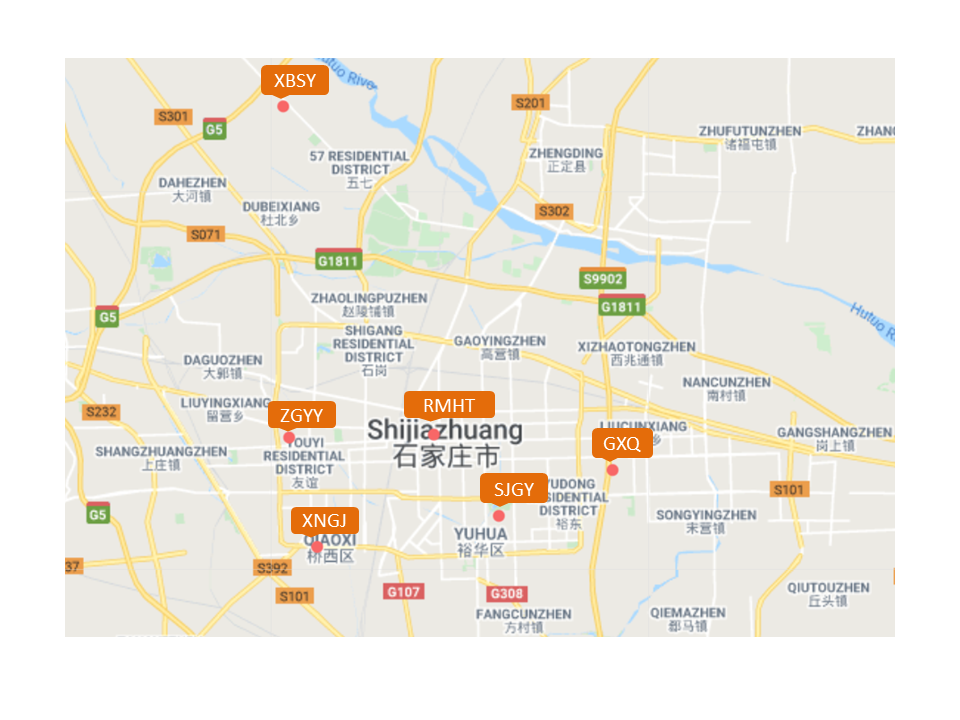
\includegraphics[width=15cm,height=10cm]{map.png}
	\caption{\footnotesize Geographic distributions of the 6 stations in Shijiazhuang. The XBSY station locates relatively far away from the other 5 stations.}
	\label{fig:map}
\end{figure}

The data are collected hourly from 2016.03.01 to 2017.02.28, including concentrations of 6 air pollutants (i.e., PM$_{2.5}$, PM$_{10}$, SO$_2$, NO$_2$, CO and O$_3$) and 5 meteorological variables (i.e., Atmospheric pressure, Temperature, Dew point, Combined wind direction and Wind speed). 

It should be noted that there are missing data in the dataset, which can be caused by having observations lower than detecting threshold or other errors in the data collection. Detailed explanations of the variables as well as their missing rate are shown in Table \ref{Tab:variable}. SO$_2$ has the highest missing rate due to its relatively low concentrations in magnitude.

\begin{table}[htbp]
	\caption{Detailed imformation and missing rate of variables observed by stations in Shijiazhuang. The missing rate is defined as the ratio of the number of missing observations over total possible number of observations for each variable. Take PM$_{2.5}$ as an example, the number of missing observations in PM$_{2.5}$ of all the 6 stations is 1290, and the number of possible observations is $N=6\times 365\times 24 =52,560$.}
	\label{Tab:variable}
	\begin{center}
		\resizebox{\textwidth}{24mm}{
			\begin{tabular}{cclcc}
				\toprule
				&\textbf{Variable} & \multicolumn{1}{c}{\textbf{Meaning}} & \textbf{Unit} & \textbf{Missing Rate(\%)}\\
				\midrule
				\multirow{6}*{\tabincell{c}{Air \\ pollutants}} & PM$_{2.5}$ & An air pollutant with a diameter of 2.5 micrometers or less & $ug/m^{3}$ & 2.45\\[3pt]
				~ & PM$_{10}$ & An air pollutant with a diameter between 2.5 and 10 micrometers & $ug/m^{3}$ & 2.43\\[3pt]
				~ & SO$_2$ & A gas produced by volcanoes and in various industrial processes & $ug/m^{3}$ & 5.40\\[3pt]
				~ & NO$_2$ & An acutely toxic reddish-brown gas with a sharp smell  & $ug/m^{3}$ & 1.30\\[3pt]
				~ & CO & A gas at room temperature produced by something organic burning & $ug/m^{3}$ & 1.32\\[3pt]		
				~ & O$_3$ &  A pale blue gas with a distinctively pungent smell & $ug/m^{3}$ & 1.21\\[3pt]				
				\midrule
				\multirow{5}*{\tabincell{c}{Meteorological \\ variables}} & atmospheric pressure & The weight of the column of air above a designated area & hPa & 1.95\\[3pt]
				~ & temperature & A measure of the hotness or coldness of the air around us & $^{\circ}C$ & 1.95\\[3pt]
				~ & dew point & The temperature to which air must be cooled for saturation to occur & $^{\circ}C$ & 1.95\\[3pt]
				~ & combined wind direction & The direction from which the wind blows & NE NW SE SW CV & 1.55\\[3pt]
				~ & wind speed & The rate of motion of air & m/s & 1.55\\[3pt]													
				\bottomrule
		\end{tabular}}
	\end{center}
\end{table}

Since the main target of our work is to automatically monitor the PM$_{2.5}$ data, we then plot the histogram of PM$_{2.5}$ concentrations of all the 6 stations in Figure \ref{fig:hist}. The histogram is highly right skewed, with mean 111.27 and median 66. 

\begin{figure}[htbp]
	\centering
	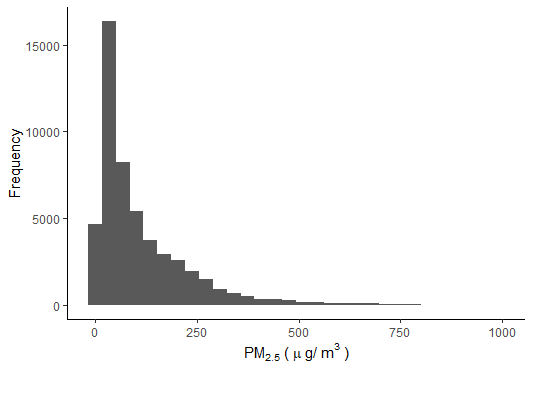
\includegraphics[width=12cm]{newhist.png}
	\caption{\footnotesize The histogram of PM$_{2.5}$ concentrations. Hourly data of 6 stations from 2016.03.01 to 2017.02.28 are combined to show.}
	\label{fig:hist}
\end{figure}

---------------------------------------------------------------------->

\scsection{Temporal Characteristics of PM$_{2.5}$}

Firstly, by season. The boxplot shows the  PM$_{2.5}$ of six stations by seasons. The right one is a time series diagram based on the average PM$_{2.5}$ of all stations per hour. 

\begin{figure}[H]
	\centering
	\subfigure[boxplot]{
		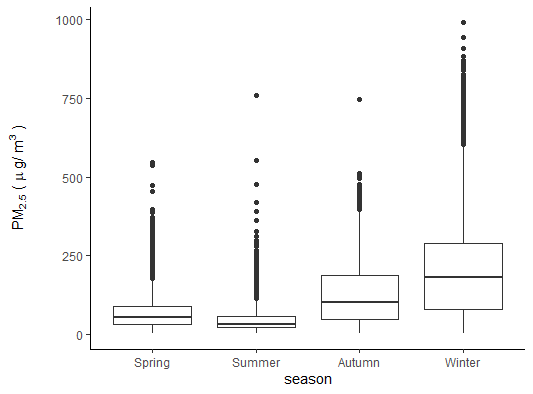
\includegraphics[width=7cm]{newseason.png}
	}
	\subfigure[time series diagram]{
		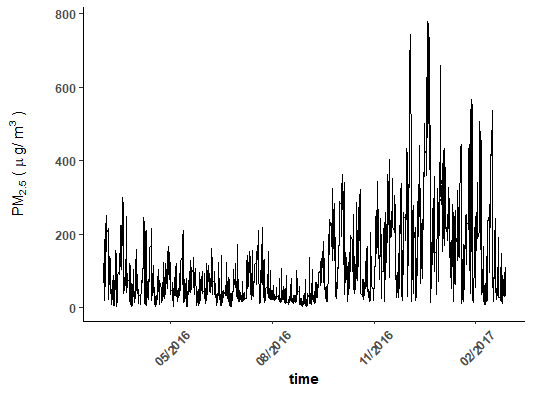
\includegraphics[width=7cm]{newts.png}
	}
	\caption{\footnotesize  Boxplot of PM$_{2.5}$ concentration of six stations by seasons and the time series diagram based on the average PM$_{2.5}$ of all stations per hour.}
	\label{fig:Seasonal trend}
\end{figure}


Secondly, by hour. The scatter plot is employed to depict the relation of concentrations of the target station between time t and time t-1 (last hour) to illustrate the temporal dependence. 

\begin{figure}[htbp]
	\centering
	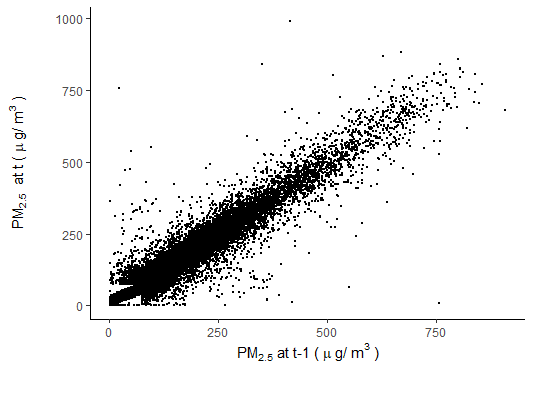
\includegraphics[width=12cm]{newtime.png}
	\caption{\footnotesize The scatter plot of PM$_{2.5}$ between adjacent times.}
	\label{fig:time}
\end{figure}


\scsection{Spatial Characteristics of PM$_{2.5}$}

The average PM$_{2.5}$ of the 6 stations separately and seasonal average value of PM2.5 for the 6 stations is shown in the table.

\begin{table}[htbp]
	\caption{Seasonal average value of PM$_{2.5}$ for the 6 stations.}
	\label{Tab:station_average}
	\begin{center}
		%\resizebox{\textwidth}{22mm}{
		\begin{tabular}{ccccccc}
			\toprule
			&\textbf{GXQ} & \textbf{RMHT} & \textbf{SJGY} & \textbf{XBSY} & \textbf{XNGJ} & \textbf{ZGYY}\\
			\midrule
			\textbf{Spring} & 67.70 & 73.88 & 72.23 & 65.55 & 62.58 & 63.14\\
			\textbf{Summer} & 44.56 & 48.83 & 50.64 & 49.63 & 48.04 & 43.79\\
			\textbf{Autumn} & 126.27 & 127.47 & 119.90 & 125.93 & 122.96 & 122.35\\
			\textbf{Winter} & 204.98 & 198.74 & 218.17 & 221.77 & 212.80 & 202.08\\
			\midrule
			\textbf{The whole year} & 110.05 & 111.83 & 113.28 & 114.97 & 110.60 & 107.01\\			
			\bottomrule
		\end{tabular}
	\end{center}
\end{table}

Accordingly, the heatmap shows seasonal average value of PM$_{2.5}$ of different stationss. 

\begin{figure}[htbp]
	\centering
	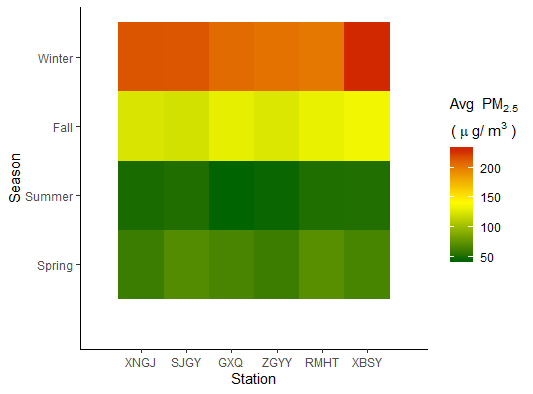
\includegraphics[]{newheatmap.png}
	\caption{\footnotesize The heatmap of the seasonal average PM$_{2.5}$ of all the 6 stations.}
	\label{fig:heatmap}
\end{figure}

The scatter plot is to depict the relation between PM$_{2.5}$ concentrations of the target station at time t and the weighted sum of concentrations of the rest of the stations at time t-1 (last hour) to illustrate the spatial dependence. The weights are proportional to the inverse of distance to the target station and sum up to 1. Figure 6 suggests that the PM$_{2.5}$ concentrations have spatial dependence.


\begin{figure}[htbp]
	\centering
	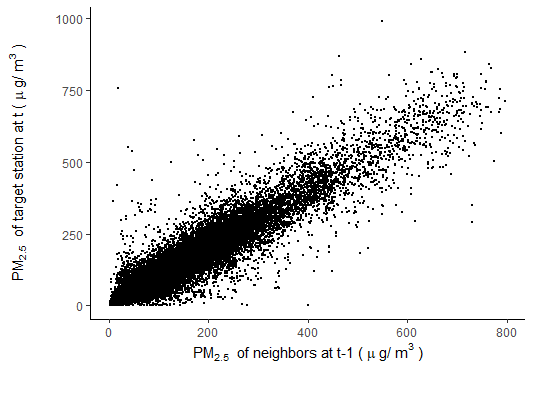
\includegraphics[width=12cm]{newspace.png}
	\caption{\footnotesize The scatter plot  between PM$_{2.5}$ concentrations of the target station at time t and the weighted sum of concentrations of the rest of the stations at time t-1.}
	\label{fig:space}
\end{figure}

-------------------------------------------------------------->

\scsection{The Meteorological Variables}

Lastly, we illustrate the distribution of meteorological variables. We bin the meteorological variables by quartiles and visualize the distributions with boxplots. Taking winter data as an example, Figure \ref{fig:meteo boxplot} shows that there is a strongly positive correlation between PM$_{2.5}$ concentrations and dew point while the correlations between PM$_{2.5}$ concentrations and atmospheric pressure, wind speed or temperature are slightly negative. PM$_{2.5}$ concentrations vary among different combined wind direction. The average of concentrations under northwest wind direction(NW) and calm wind(CV) are the two highest. The correlation coefficients between PM$_{2.5}$ concentrations and dew point, atmospheric pressure, wind speed or temperature are 0.56, -0.30, -0.25, -0.17. Therefore, we include these meteorological variables into the regression models so as to eliminate the impact brought about by these variables.

\begin{figure}[htbp]
	\centering
	\subfigure[atmospheric pressure]{
		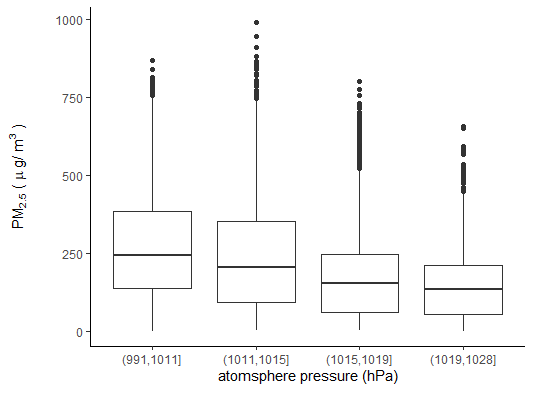
\includegraphics[width=7cm]{newpressure.png}
	}
	\subfigure[temperature]{
		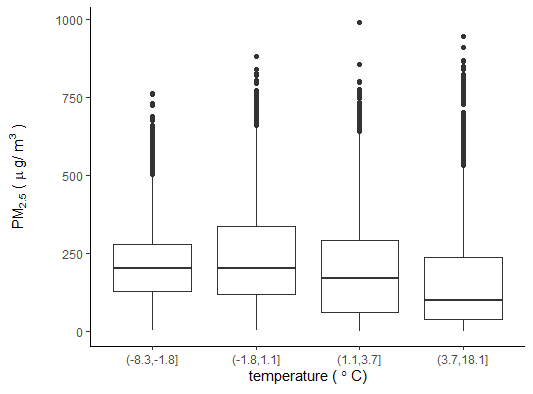
\includegraphics[width=7cm]{newtemp.png}
	}
	
	\subfigure[dew point]{
		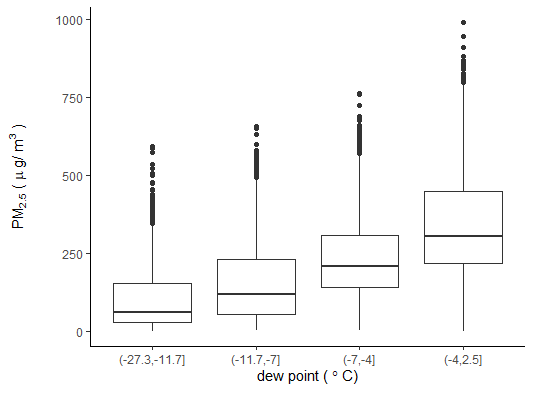
\includegraphics[width=7cm]{newdewp.png}
	}
	\subfigure[wind speed]{
		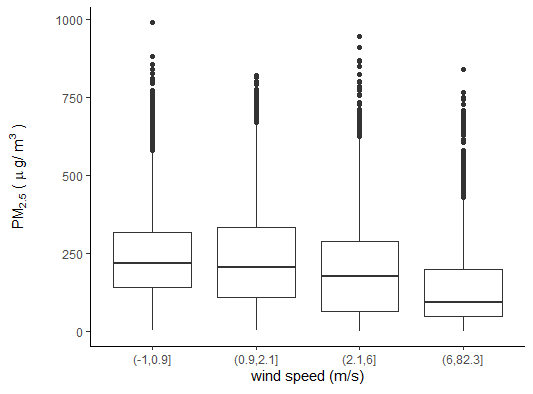
\includegraphics[width=7cm]{newiws.png}
	}
	
	\subfigure[combined wind direction]{
		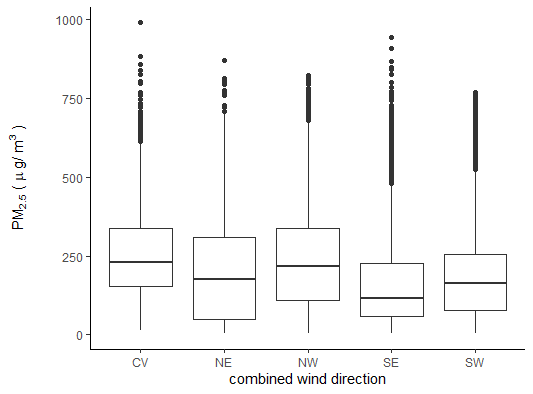
\includegraphics[width=7cm]{newcbwd.png}
	}
	\caption{\footnotesize  Boxplots of PM$_{2.5}$ concentrations and some meteorological variables. Winter data is chosen for instance.}
	\label{fig:meteo boxplot}
\end{figure}


\newpage
------------------------------

(Professor Pan asked us to put it in the model part. So it's here for the time being)

We further calculate ACF and PACF based on the time series of PM$_{2.5}$ concentrations  in Figure \ref{fig:ACFPACF} to illustrate the temporal dependence. ACF shows slow decay while Partial ACF is truncated with a large value at lag 1, which suggests to fit an AR(1) model. 

\begin{figure}[htbp]
	\centering
	\subfigure[acf]{
		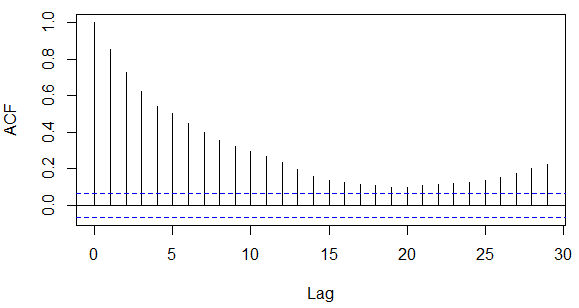
\includegraphics[width=7cm]{acf.png}
	}
	\subfigure[pacf]{
		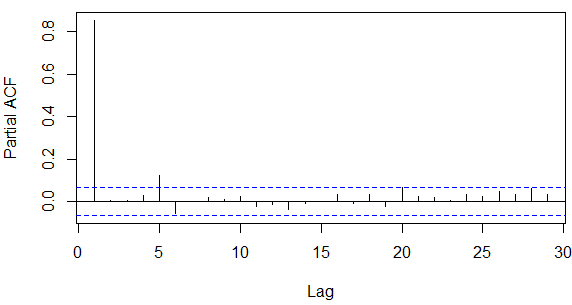
\includegraphics[width=7cm]{pacf.png}
	}
	\caption{\footnotesize ACF and PACF of PM$_{2.5}$ concentrations time series. A piece of continuous data without missing(GaoXinQu 2017.07.24-2017.08.31) is chosen for instance.}
	\label{fig:ACFPACF}
\end{figure}

\newpage

\bibliography{reference}
\end{document}
